\documentclass{article}

\usepackage{url}
\usepackage{graphicx}

\title{Drawing Trees and Animating Tree Changes}

\author{Sandro Badame, Peter Boothe$^*$\\
 Manhattan College\\
\url{{sbadame.student,peter.boothe}@manhattan.edu}}

\newcommand{\newword}[1]{\textit{#1}\index{#1}}
\newcommand{\java}[1]{\texttt{#1}\index{#1}}

\begin{document}
\maketitle

\begin{abstract}
Dynamic trees appear in many areas of computer science, including, but not
limited to, Lisp code, data structures, tree automata, and computer
algorithms.  It would be useful to be able to easily draw trees and animate
them changing over time.  We begin by articulating a design for tree
visualization and animation that is more general than previous methodologies.
We demonstrate, using several visualizations, the
usage of a library we have created which attempts to simplify the graphics
aspect of this tricky task.\end{abstract}

\section{Introduction}
Trees, and especially trees which change over time, are fundamental objects in
computer science.  They occur in many disparate contexts, and while the uses of
these trees may be different, there are some commonalities which we can use to
build a tree visualization system which might be useful in many different
contexts.  In this paper we articulate the design principles of a general tree visualization system, present one such system that we have built in Java and made freely available, and then demonstrate our system's utility with several sample visualizations.

There are multiple reasons to visualize a system, and different reasons have
different requirements for the visualization.  A visualization designed for
experts may be very useful for that target group, but leave neophytes
confused.  Therefore, before we discuss the particulars of our visualization,
we must explain our reasons for wanting such a system in the first place, and
the expected audience.  We want to visualize dynamic trees for demonstration,
education, and beauty, and we would like our visualizations to be of benefit to
computer science undergraduates.

\subsection{Visualization for Demonstration}

We want to show them how things work.  We therefore will restrict ourselves to trees which are small enough to be drawn in their entirety on a single computer screen.

\subsection{Visualization for Education}

It turns out that demonstrations are often useless.  But if we force students to build their own visualizations, then they actually learn.  So We would like to enable that as well.

\subsection{Visualization for Beauty}

Computational processes are often both sophisticated and beautiful, but their
beauty is often lost in the nitty-gritty of simply getting a given algorithm to
work.  Using a visualization system could, hopefully, remind students of the
beauty of the structures they are working with and also serve as an effective
advertisement to non-majors of the intricacy and interestingness available in
the CS major.

\section{Designing a Tree Visualization Framework}

Let us begin our design by formally defining the objects under consideration.
A \newword{tree} $T$ is an undirected connected acyclic graph with vertex set
$V$ and edge set $E \subseteq \{V \times V\}$.  A \newword{rooted tree} is a
tree where a particular vertex $r$ is designated the as the \newword{root} of
the tree, which allows us to define the \newword{depth} of a vertex $v$ as the
length of the shortest path between $v$ and $r$. Every edge connects two
vertices $(u,v)$, and we will assume, again wlog, that the depth of $u$ is one
less than the depth of $v$.  In that case, we call $u$ the \newword{parent} of
$v$ and $v$ the \newword{child} of $u$.  The \newword{children} of $v$ are the
set of vertices which have $v$ as their parent.  A \newword{rooted ordered
tree} is a rooted tree with a partial-ordering on the vertex set $V$ such that
for all vertices $\{u,v, \ldots\}$ with the same parent, either $u < v$ or $v <
u$.  

Without loss of generalization, we restrict our visualization system to rooted,
ordered trees.  Any tree can be converted into a rooted, ordered tree by
selecting a root and imposing a partial-ordering on the vertices.  In practice,
however, we found that every domain we considered had a naturally occuring root
and ordering, and that the imposition of an arbitrary root and ordering was
unnecessary.  From now on, when we say tree, we will mean a rooted ordered tree.

To lay out a tree in the plane, we must map every vertex $v \in V$ to a
coordinate $(v_x, v_y)$.  When visualizing a tree we put the root at the top
(which, while counter-intuitive for biologists, is standard practice in
computer science), and every vertex $\{u,v \ldots\} \subset V$ with equal depth
should be laid out with the same $y$-coordinate $(u_y = v_y)$.  Furthermore, if
two nodes $u$ and $v$ have the same parent and $u < v$, then we should lay them
out with $u_x < v_x$, which will preserve in our layout the natural order of the tree.  Our last requirement is that if we have two nodes $w$ and $z$ with equal depth and children $U$ and $V$, and $w_x < z_x$, then $u_x < v_x \forall u\in U, v\in V$.  This last requirement allows us to avoid crossing edges.

\subsection{Prior Work}

Paper from 1996 and Tamassia and the force-directed placement algorithm\cite{fdp}.

\subsection{Taking Advantage of Computational Abundance}

Past visualization frameworks went to great lengths to articulate the allowed
set of transformations which allowed them to heavily optimize their layout code
to minimize CPU usage.  In our situation, we would like to make our library as
usable as possible.  Therefore, we take every possible opportunity to make our
library easy to use, even if it increases the polynomial runtime of some of our
methods.  This is safe to do because we have restricted ourself to those graphs
which can be drawn, in their entirety, on a computer screen, and have therefore
restricted ourself to the (admittedly ill-defined) set of graphs which are
``small enough'' to still be drawn quickly using algorithms which may be of
order $\Omega(n^2)$, as long as these algorithms are not super-polynomial.

Therefore, instead of restricting ourself to a particular subset of allowed
tree operations, we allow arbitrary transformations of the tree, and then we
animate our old tree transforming into the new tree.

\subsection{Layout Algorithm}

1) Fix the root node to the middle top position. 
2) For each node of a given level treat every 
link as a spring and every node as a magnet 
and calculate the resultant forces. 
3) Simulate the change in position due to 
these forces and update all node positions 
by a small amount. 
4) Display the system to the user, and repeat 

\subsection{Animation Algorithm}

Either on every tree transformation, or when requested by the visualization programmer, we relayout the entire tree according to our layout algorithm, and then we animate the transition from the older, currently-laid-out tree, to the new tree.  Or animation proceeds in the following steps:

1) Layout the new tree using the method above. 
Do this layout off screen. 
2) Fade out any of the nodes of the currently 
displayed original tree that have been removed. 
3) Compare the locations of the nodes in the 
original tree to those in the new tree, then 
animate the movement of the original nodes 
to their new positions. 
4) Fade in any nodes that only exist in the 
new tree. 
Multiple changes can be either combined into a 
single animation step, or each step may be 
animated individually.  This allows artistic flexibility 
when creating a new visualization. 

\section{Our Library}

Our library is written in Java, and users of the library need only use two of the classes it contains: the \java{Tree} class, and the \java{TreeDisplay} class.  
\subsection{How-To}

The class \java{TreeDisplay} needs to only be created once.  A \java{TreeDisplay} may be used a GUI element for any code.

\subsection{A Sample Application}

\section{Example Animations}
\subsection{Random Tree Growth}
\subsection{Self-Balancing Binary Search Tree}
\subsection{Tree Automaton}
\begin{figure}
\begin{center}
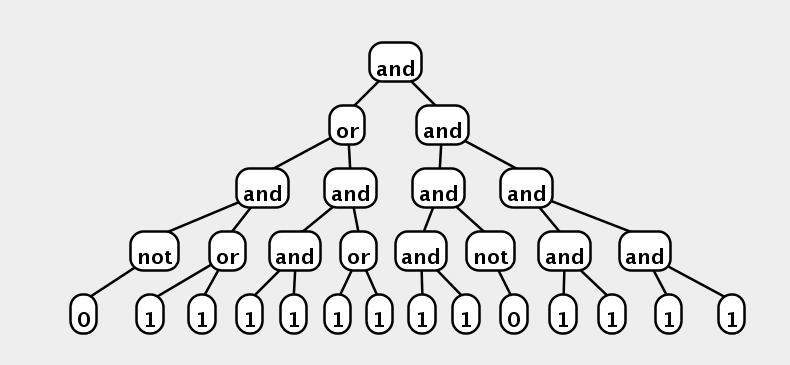
\includegraphics[width=1in]{../board/pics/ss301.png}
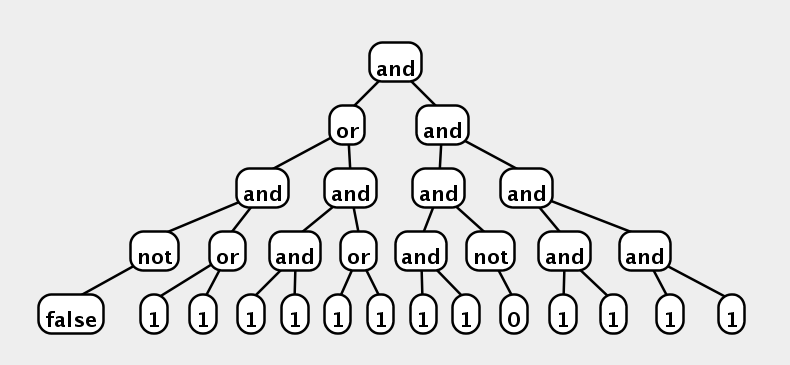
\includegraphics[width=1in]{../board/pics/ss351.png}
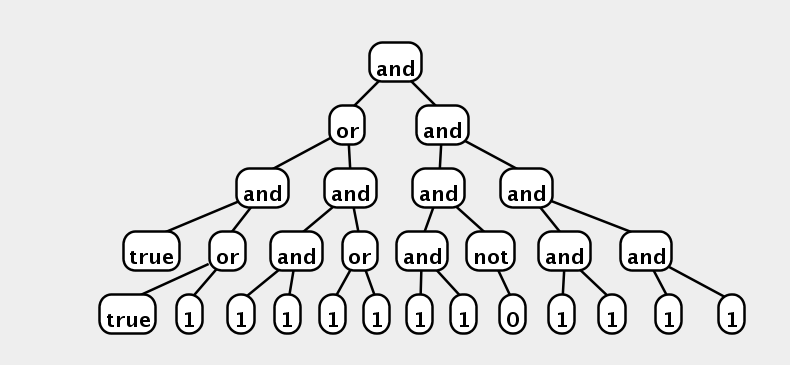
\includegraphics[width=1in]{../board/pics/ss401.png}
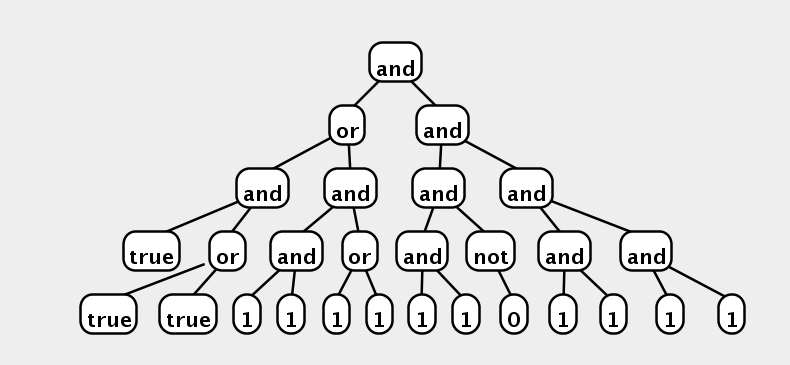
\includegraphics[width=1in]{../board/pics/ss451.png}
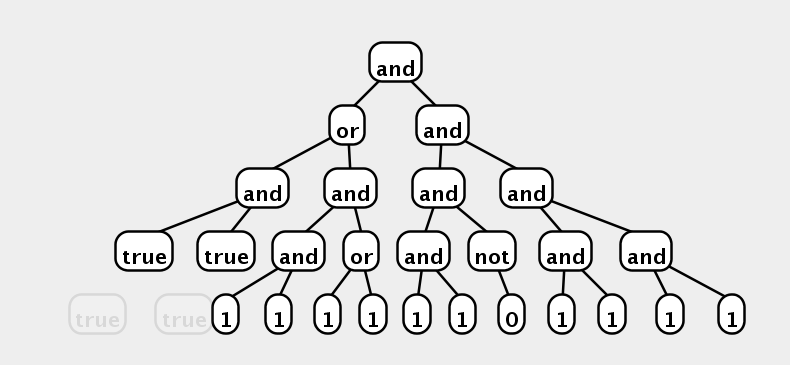
\includegraphics[width=1in]{../board/pics/ss501.png}
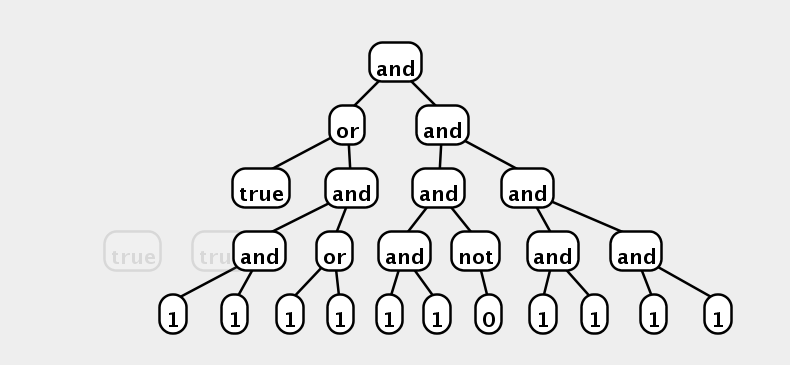
\includegraphics[width=1in]{../board/pics/ss551.png}
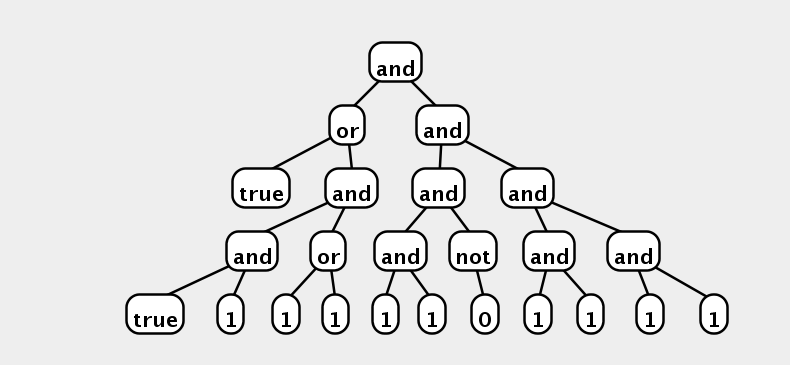
\includegraphics[width=1in]{../board/pics/ss601.png}
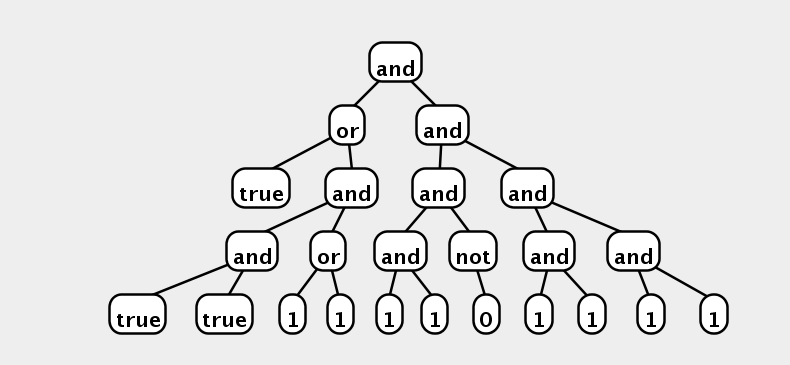
\includegraphics[width=1in]{../board/pics/ss651.png}
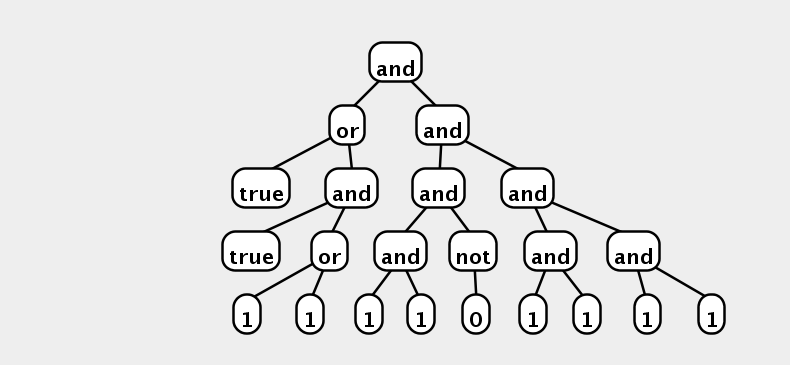
\includegraphics[width=1in]{../board/pics/ss701.png}
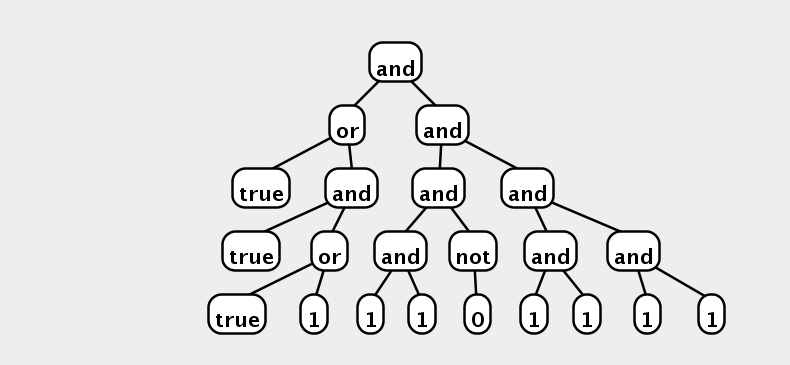
\includegraphics[width=1in]{../board/pics/ss751.png}
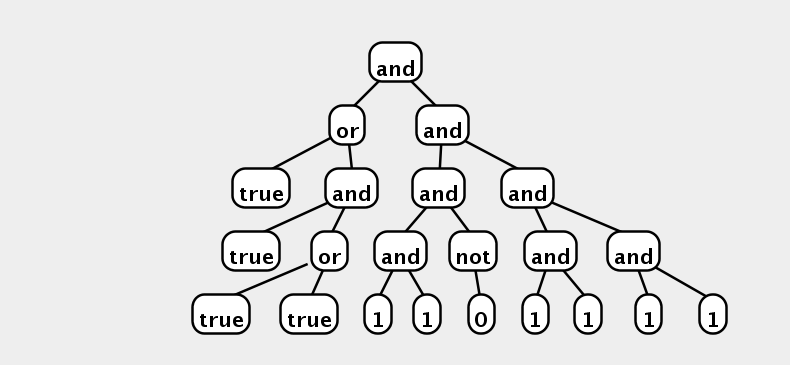
\includegraphics[width=1in]{../board/pics/ss801.png}
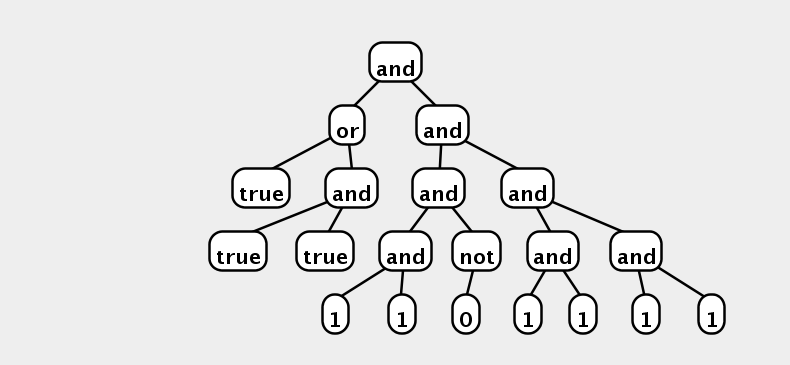
\includegraphics[width=1in]{../board/pics/ss851.png}
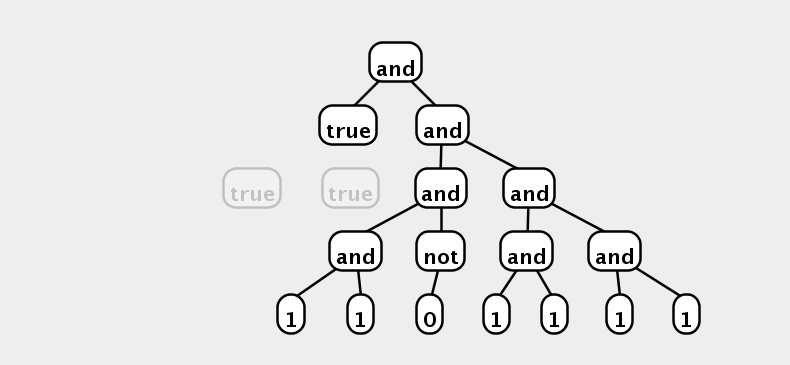
\includegraphics[width=1in]{../board/pics/ss901.png}
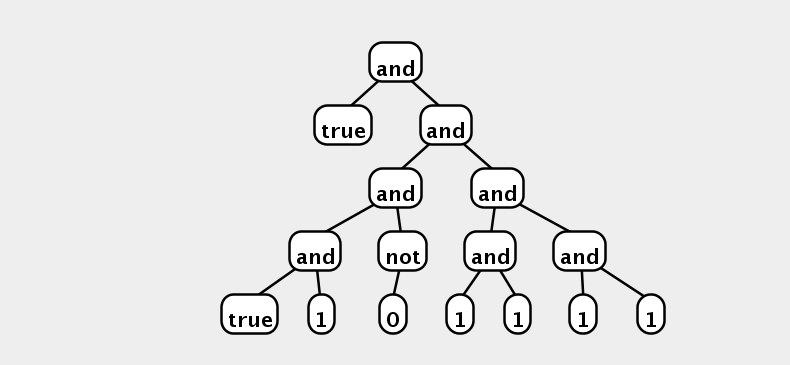
\includegraphics[width=1in]{../board/pics/ss951.png}
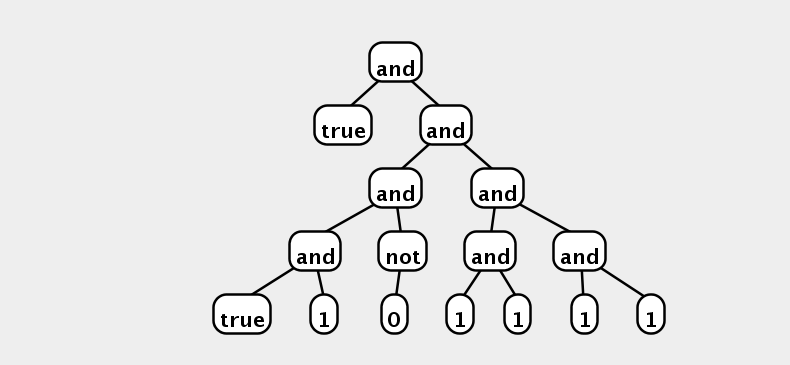
\includegraphics[width=1in]{../board/pics/ss1001.png}
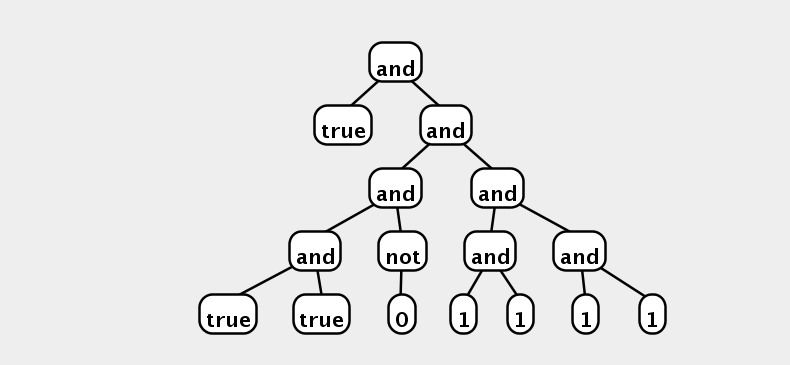
\includegraphics[width=1in]{../board/pics/ss1051.png}
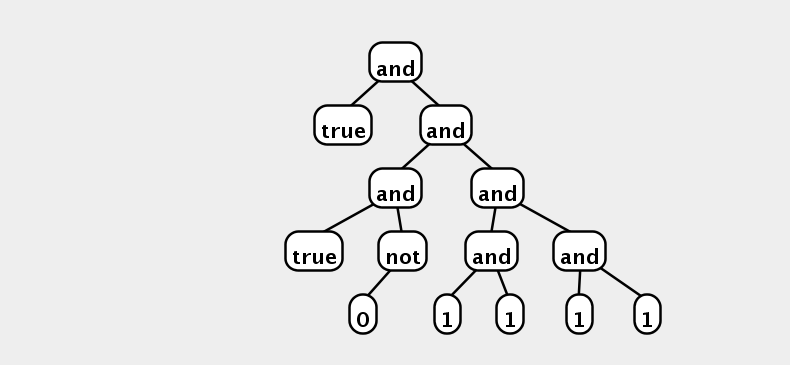
\includegraphics[width=1in]{../board/pics/ss1101.png}
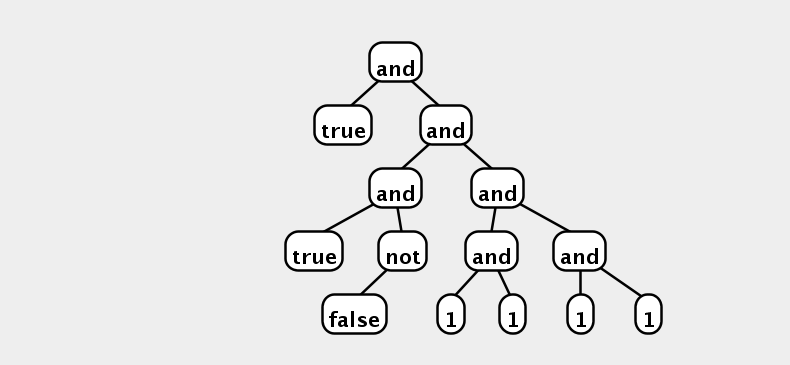
\includegraphics[width=1in]{../board/pics/ss1151.png}
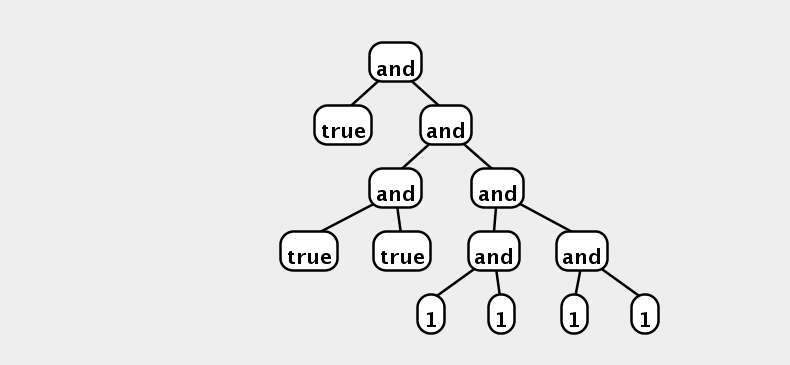
\includegraphics[width=1in]{../board/pics/ss1201.png}
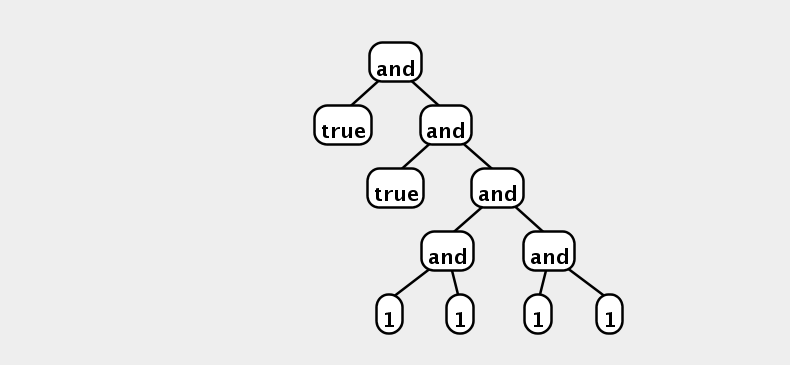
\includegraphics[width=1in]{../board/pics/ss1251.png}
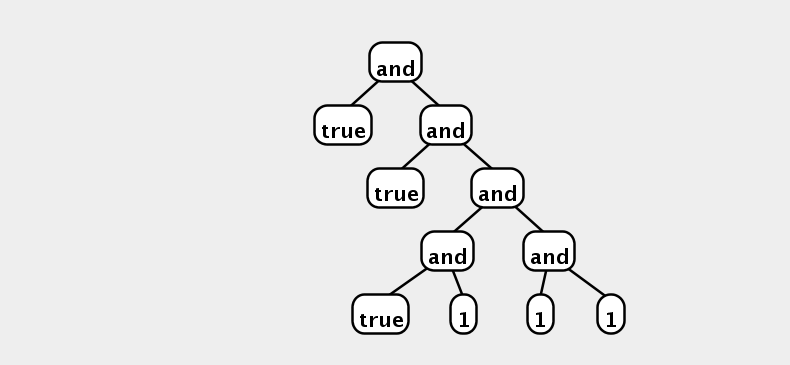
\includegraphics[width=1in]{../board/pics/ss1301.png}
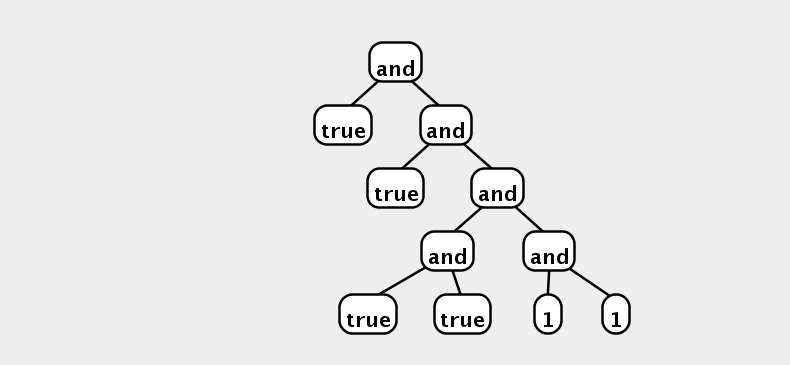
\includegraphics[width=1in]{../board/pics/ss1351.png}
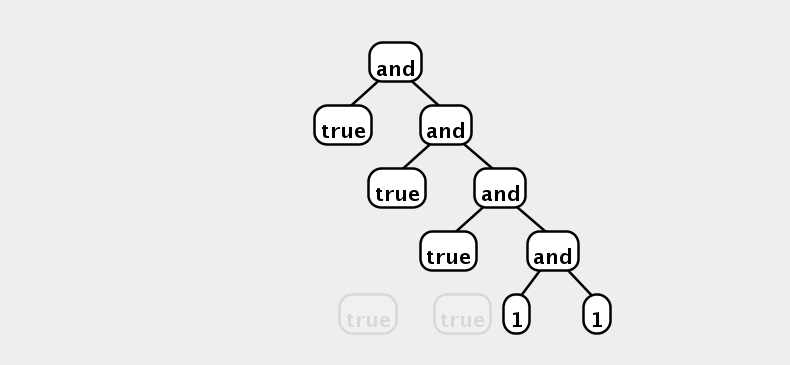
\includegraphics[width=1in]{../board/pics/ss1401.png}
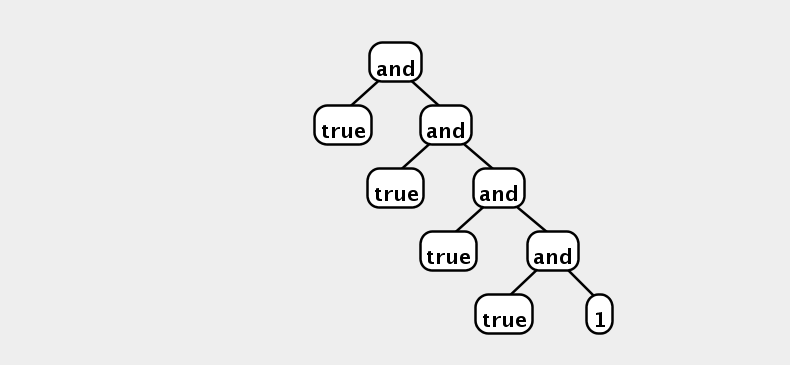
\includegraphics[width=1in]{../board/pics/ss1451.png}
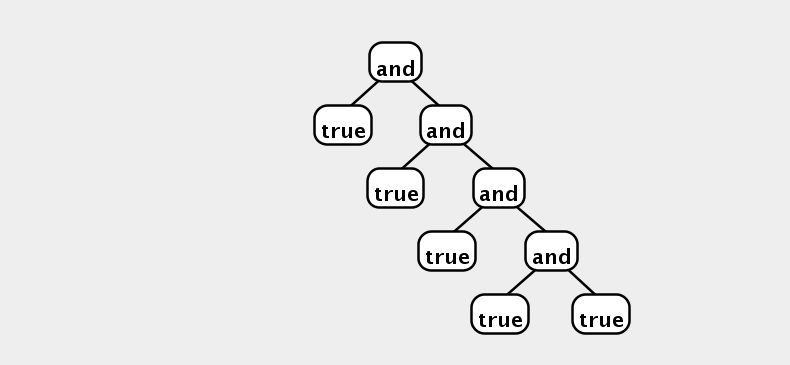
\includegraphics[width=1in]{../board/pics/ss1501.png}
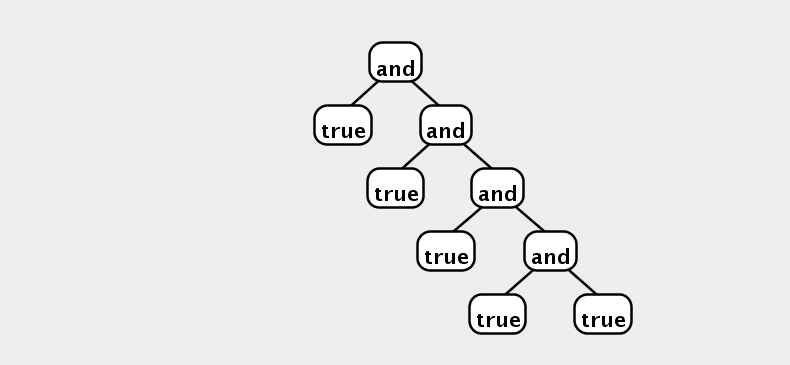
\includegraphics[width=1in]{../board/pics/ss1551.png}
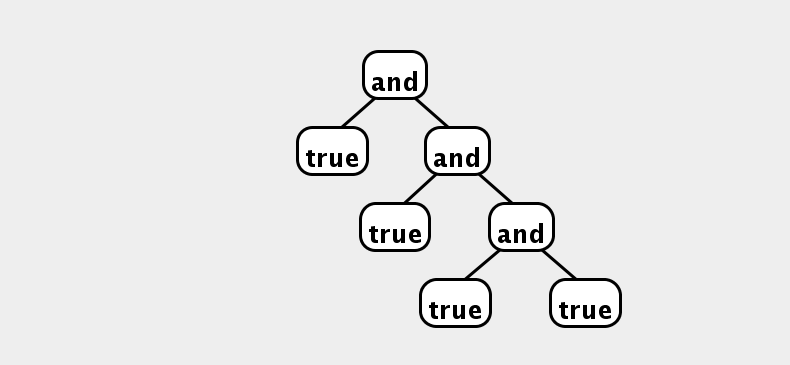
\includegraphics[width=1in]{../board/pics/ss1601.png}
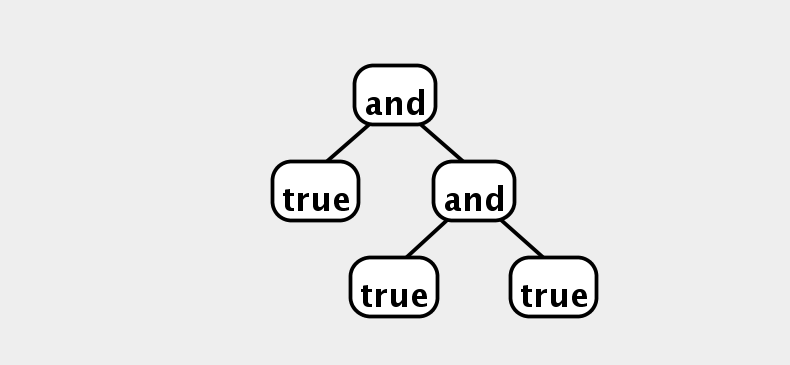
\includegraphics[width=1in]{../board/pics/ss1651.png}
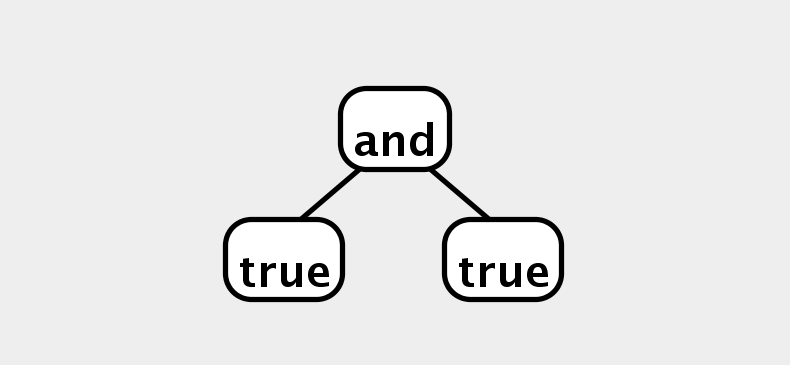
\includegraphics[width=1in]{../board/pics/ss1701.png}

\includegraphics[width=1in]{../board/pics/ss1751.png}

\includegraphics[width=1in]{../board/pics/ss1801.png}
\end{center}
\caption{Execution of a tree automaton which recognizes tautologies}
\end{figure}


\subsection{Lisp}

\begin{figure}
\begin{center}
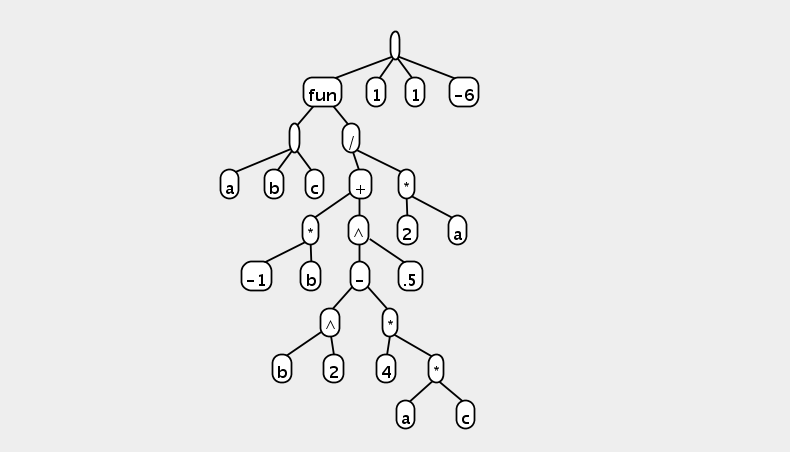
\includegraphics[width=1.25in]{../board/pics/qf1101.png}
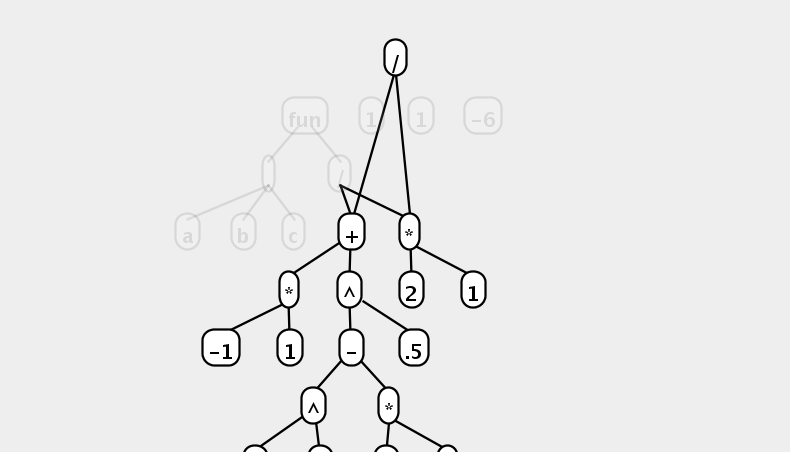
\includegraphics[width=1.25in]{../board/pics/qf1551.png}
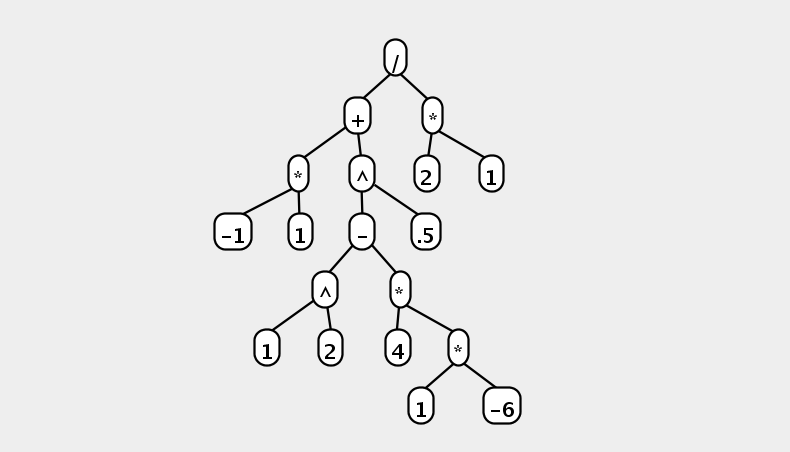
\includegraphics[width=1.25in]{../board/pics/qf1601.png}
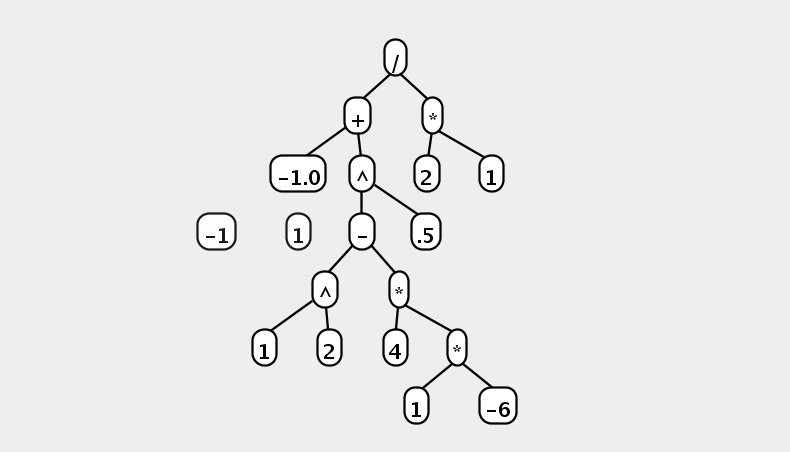
\includegraphics[width=1.25in]{../board/pics/qf1651.png}
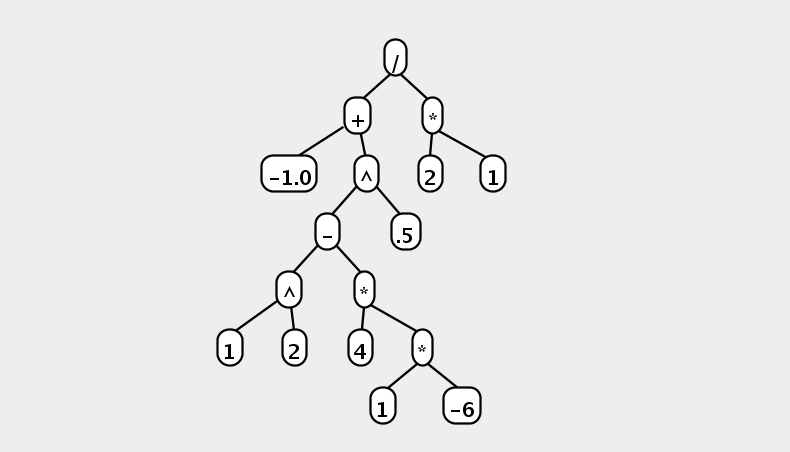
\includegraphics[width=1.25in]{../board/pics/qf1701.png}
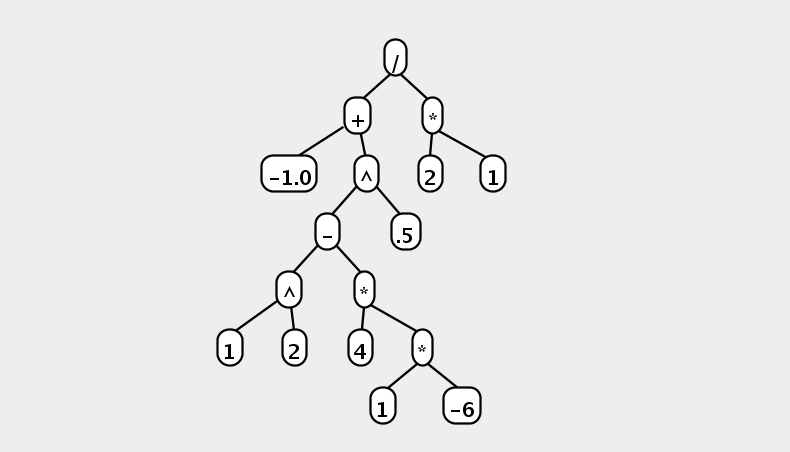
\includegraphics[width=1.25in]{../board/pics/qf1801.png}
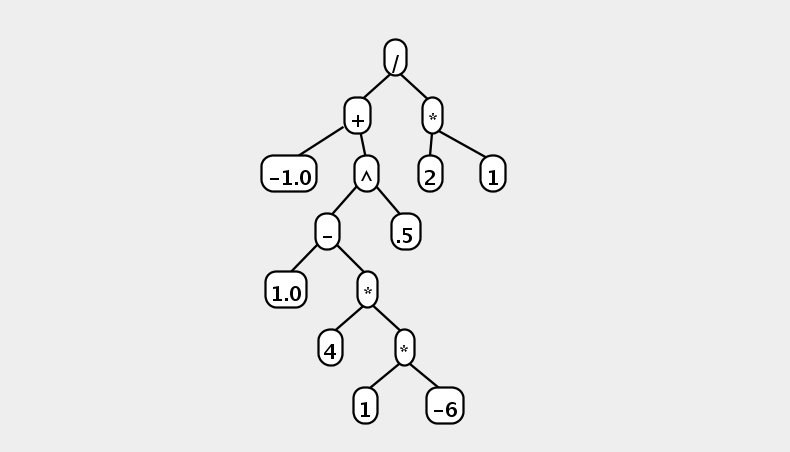
\includegraphics[width=1.25in]{../board/pics/qf1951.png}
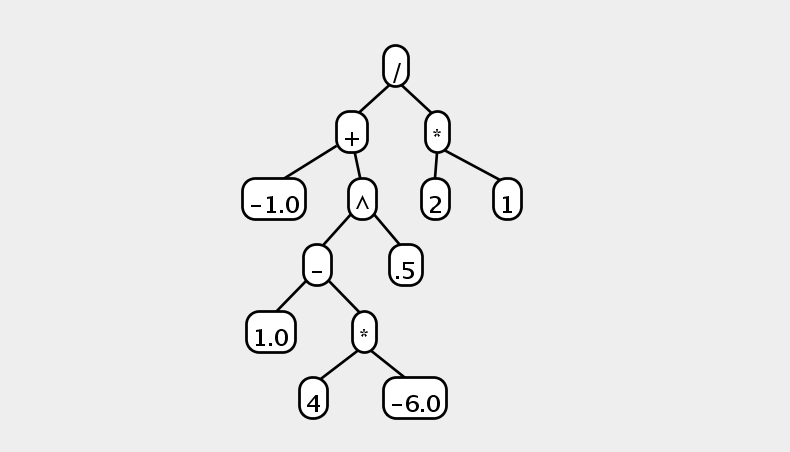
\includegraphics[width=1.25in]{../board/pics/qf2001.png}
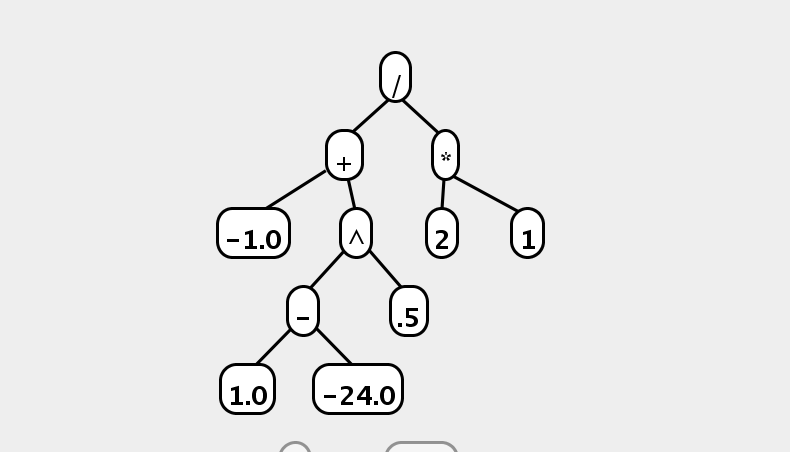
\includegraphics[width=1.25in]{../board/pics/qf2101.png}
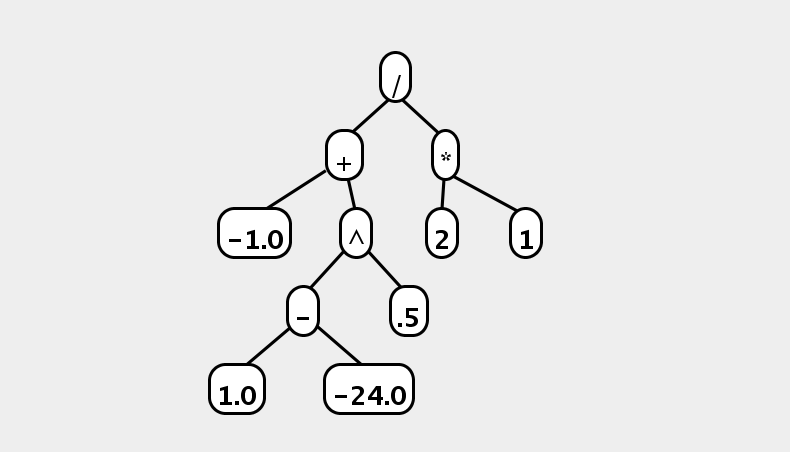
\includegraphics[width=1.25in]{../board/pics/qf2151.png}
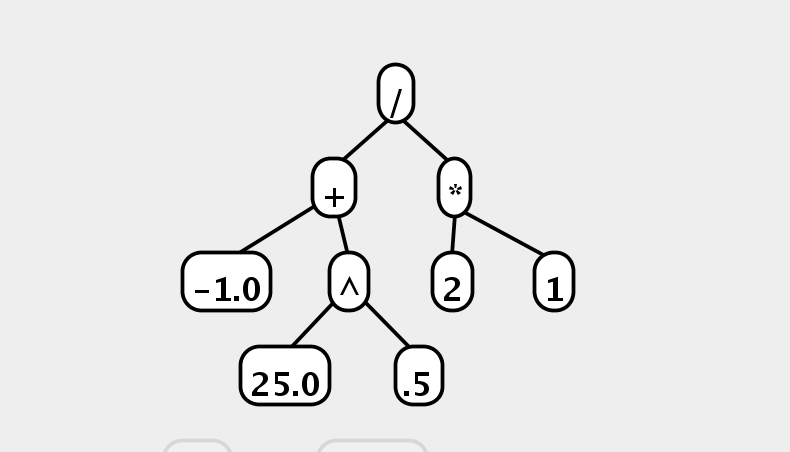
\includegraphics[width=1.25in]{../board/pics/qf2251.png}
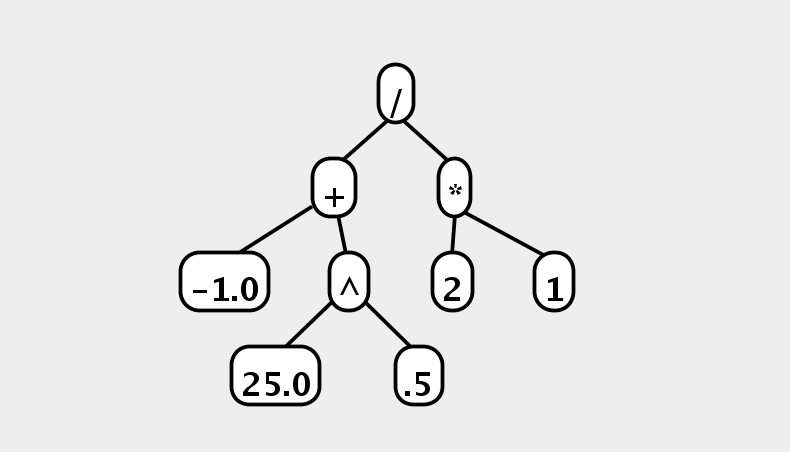
\includegraphics[width=1.25in]{../board/pics/qf2301.png}
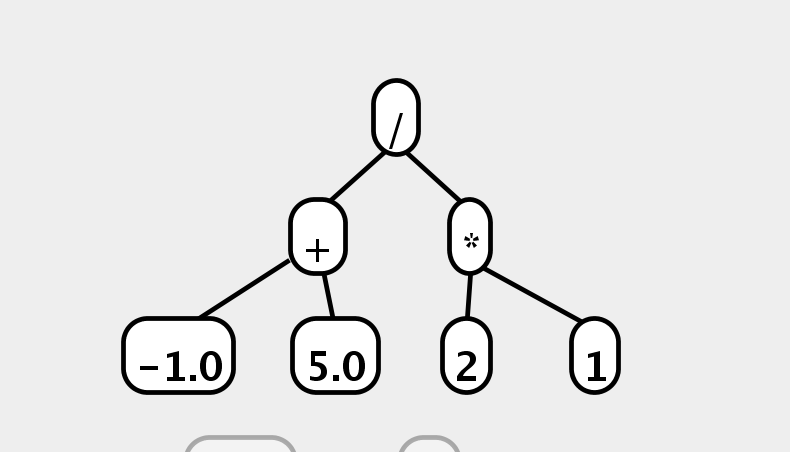
\includegraphics[width=1.25in]{../board/pics/qf2351.png}
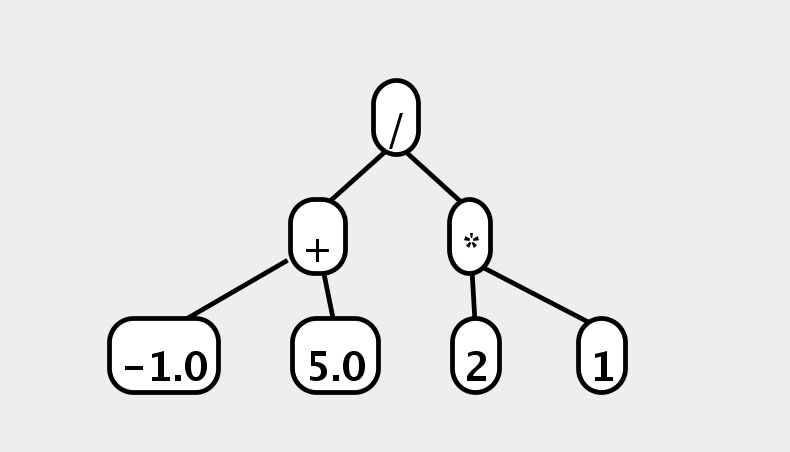
\includegraphics[width=1.25in]{../board/pics/qf2401.png}
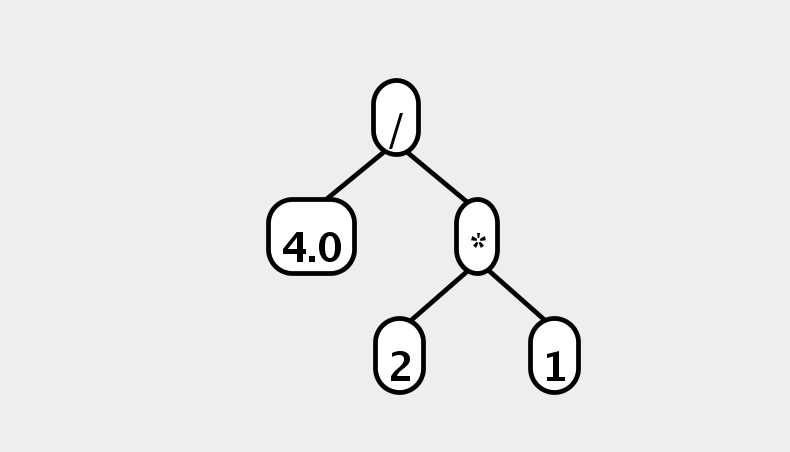
\includegraphics[width=1.25in]{../board/pics/qf2551.png}
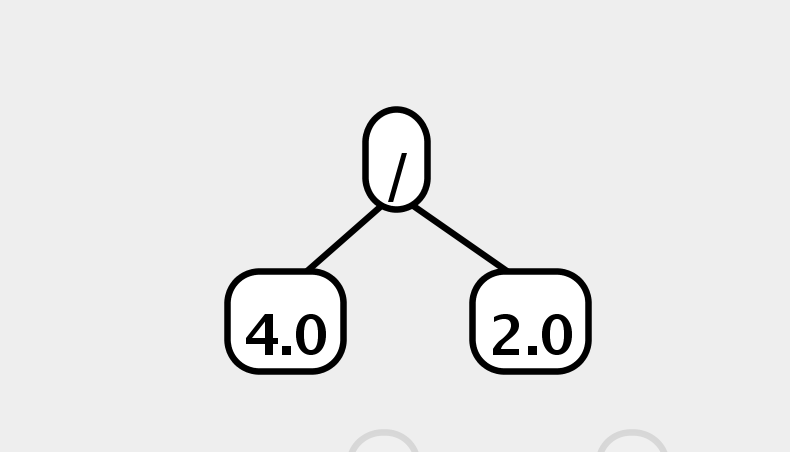
\includegraphics[width=1.25in]{../board/pics/qf2601.png}
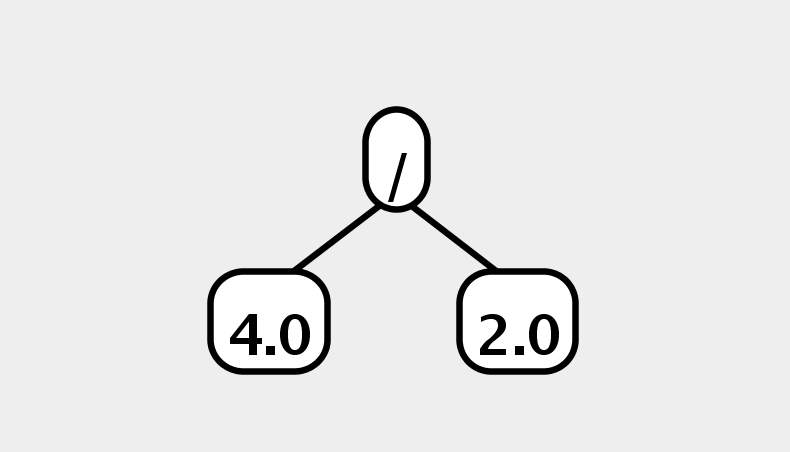
\includegraphics[width=1.25in]{../board/pics/qf2701.png}
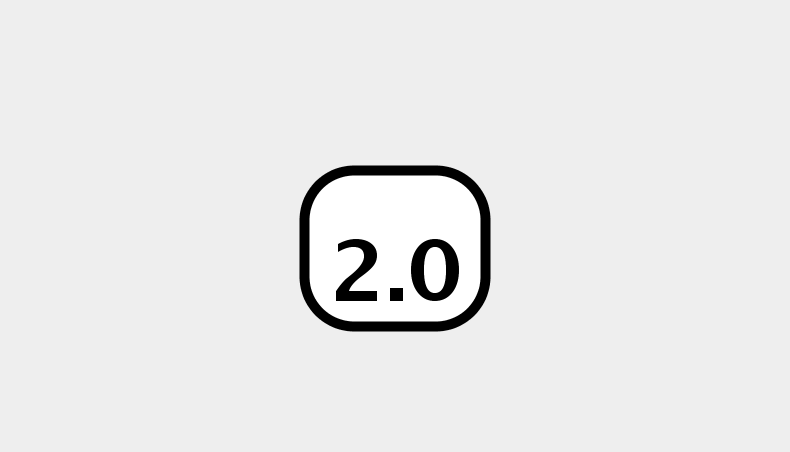
\includegraphics[width=1.25in]{../board/pics/qf2801.png}
\end{center}
\caption{The complete execution of a lisp program calculating one of the roots of $x^2+x-6$.}
\end{figure}


\section{Conclusion}

We have passed a threshold of computational abundance which can allow visualization libraries to use less-efficient algorithms in pursuit of programming ease.  Noting this threshold allows us to articulate a design for a layout library that, by doing much more work behind the scenes, makes the creation and usage of visualizations available to a much larger audience.  We have created such a library and provided several sample visualizations.  We hope that any and all of our design ideas, the resulting library, and the provided visualizations, might be useful to others who are attempting to demonstrate, learn, understand, or admire the behavior of trees which evolve over time.

\bibliographystyle{plain}
\bibliography{bibliography.bib}

\end{document}
